%!TeX root=../pridetop.tex
\chapter[Chapter \thechapter]{}
	
\begin{figure}[t!]
\centering
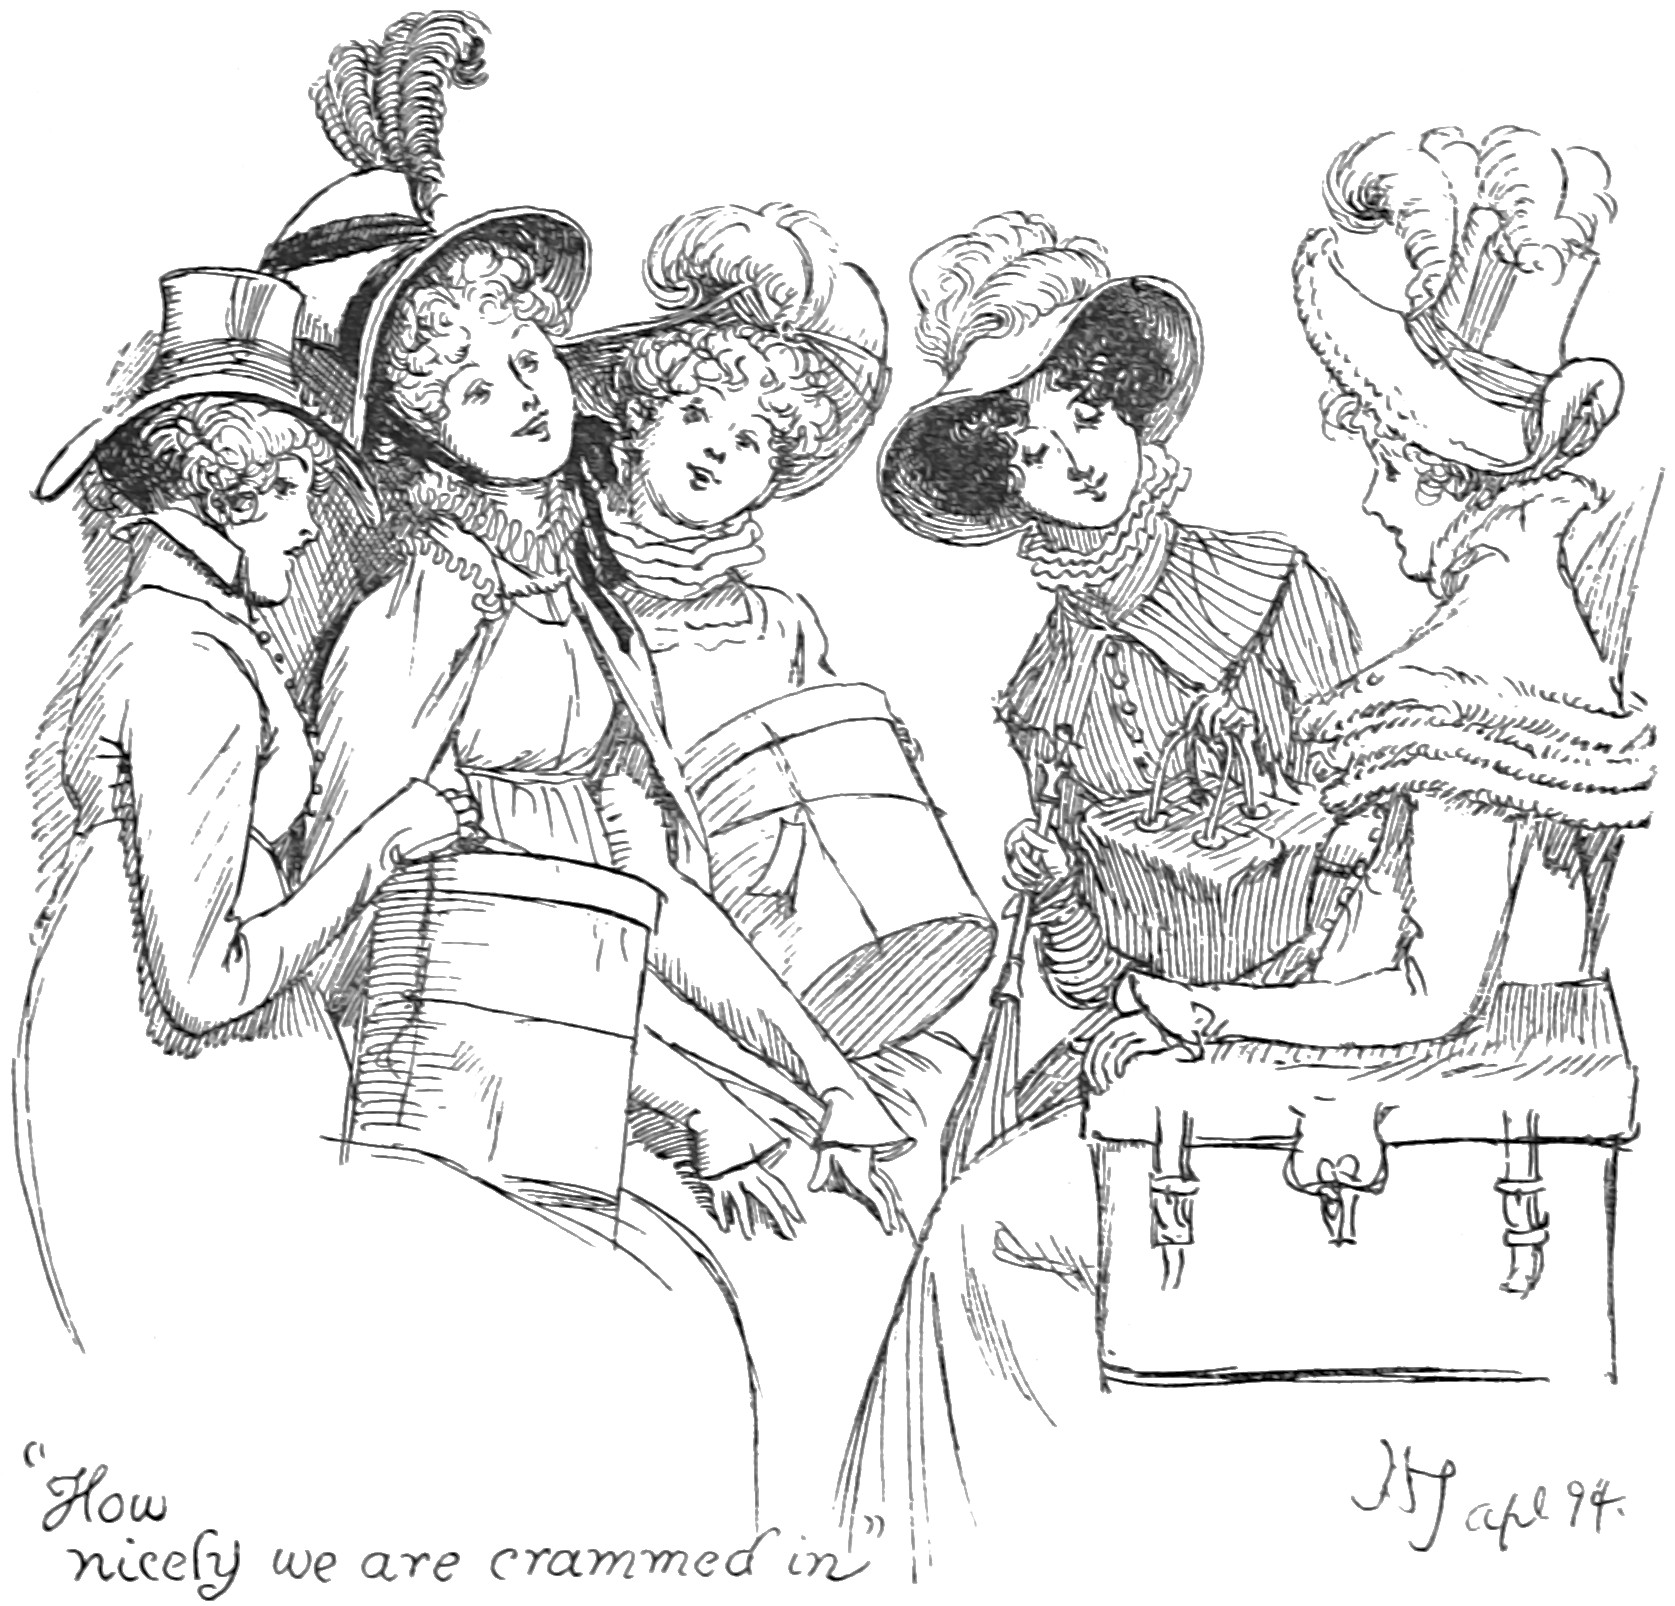
\includegraphics[width=\linewidth]{39top}
\captionlistentry{»How nicely we are crammed in!«}
\end{figure}


\lettrine[lines=6,image=true,findent=2pt]{initials/chap39it}{ was} the second week in May, in which the three young ladies set out together from Gracechurch Street for the town of ——, in Hertfordshire; and, as they drew near the appointed inn where Mr Bennet's carriage was to meet them, they quickly perceived, in token of the coachman's punctuality, both Kitty and Lydia looking out of a dining-room upstairs. These two girls had been above an hour in the place, happily employed in visiting an opposite milliner, watching the sentinel on guard, and dressing a salad and cucumber.

After welcoming their sisters, they triumphantly displayed a table set out with such cold meat as an inn larder usually affords, exclaiming, »Is not this nice? is not this an agreeable surprise?«

»And we mean to treat you all,« added Lydia; »but you must lend us the money, for we have just spent ours at the shop out there.« Then showing her purchases,—»Look here, I have bought this bonnet. I do not think it is very pretty; but I thought I might as well buy it as not. I shall pull it to pieces as soon as I get home, and see if I can make it up any better.«

And when her sisters abused it as ugly, she added, with perfect unconcern, »Oh, but there were two or three much uglier in the shop; and when I have bought some prettier-coloured satin to trim it with fresh, I think it will be very tolerable. Besides, it will not much signify what one wears this summer, after the ——shire have left Meryton, and they are going in a fortnight.«

»Are they, indeed?« cried Elizabeth, with the greatest satisfaction.

»They are going to be encamped near Brighton; and I do so want papa to take us all there for the summer! It would be such a delicious scheme, and I dare say would hardly cost anything at all. Mamma would like to go, too, of all things! Only think what a miserable summer else we shall have!«

»Yes,« thought Elizabeth; »\textit{that} would be a delightful scheme, indeed, and completely do for us at once. Good Heaven! Brighton and a whole campful of soldiers, to us, who have been overset already by one poor regiment of militia, and the monthly balls of Meryton!«

»Now I have got some news for you,« said Lydia, as they sat down to table. »What do you think? It is excellent news, capital news, and about a certain person that we all like.«

Jane and Elizabeth looked at each other, and the waiter was told that he need not stay. Lydia laughed, and said,—

»Ay, that is just like your formality and discretion. You thought the waiter must not hear, as if he cared! I dare say he often hears worse things said than I am going to say. But he is an ugly fellow! I am glad he is gone. I never saw such a long chin in my life. Well, but now for my news: it is about dear Wickham; too good for the waiter, is not it? There is no danger of Wickham's marrying Mary King—there's for you! She is gone down to her uncle at Liverpool; gone to stay. Wickham is safe.«

»And Mary King is safe!« added Elizabeth; »safe from a connection imprudent as to fortune.«

»She is a great fool for going away, if she liked him.«

»But I hope there is no strong attachment on either side,« said Jane.

»I am sure there is not on \textit{his}. I will answer for it, he never cared three straws about her. Who \textit{could} about such a nasty little freckled thing?«

Elizabeth was shocked to think that, however incapable of such coarseness of \textit{expression} herself, the coarseness of the \textit{sentiment} was little other than her own breast had formerly harboured and fancied liberal!

As soon as all had ate, and the elder ones paid, the carriage was ordered; and, after some contrivance, the whole party, with all their boxes, workbags, and parcels, and the unwelcome addition of Kitty's and Lydia's purchases, were seated in it.

»How nicely we are crammed in!« cried Lydia. »I am glad I brought my bonnet, if it is only for the fun of having another band-box! Well, now let us be quite comfortable and snug, and talk and laugh all the way home. And in the first place, let us hear what has happened to you all since you went away. Have you seen any pleasant men? Have you had any flirting? I was in great hopes that one of you would have got a husband before you came back. Jane will be quite an old maid soon, I declare. She is almost three-and-twenty! Lord! how ashamed I should be of not being married before three-and-twenty! My aunt Philips wants you so to get husbands you can't think. She says Lizzy had better have taken Mr Collins; but \textit{I} do not think there would have been any fun in it. Lord! how I should like to be married before any of you! and then I would \textit{chaperon} you about to all the balls. Dear me! we had such a good piece of fun the other day at Colonel Forster's! Kitty and me were to spend the day there, and Mrs Forster promised to have a little dance in the evening; (by-the-bye, Mrs Forster and me are \textit{such} friends!) and so she asked the two Harringtons to come: but Harriet was ill, and so Pen was forced to come by herself; and then, what do you think we did? We dressed up Chamberlayne in woman's clothes, on purpose to pass for a lady,—only think what fun! Not a soul knew of it, but Colonel and Mrs Forster, and Kitty and me, except my aunt, for we were forced to borrow one of her gowns; and you cannot imagine how well he looked! When Denny, and Wickham, and Pratt, and two or three more of the men came in, they did not know him in the least. Lord! how I laughed! and so did Mrs Forster. I thought I should have died. And \textit{that} made the men suspect something, and then they soon found out what was the matter.«

With such kind of histories of their parties and good jokes did Lydia, assisted by Kitty's hints and additions, endeavour to amuse her companions all the way to Longbourn. Elizabeth listened as little as she could, but there was no escaping the frequent mention of Wickham's name.

Their reception at home was most kind. Mrs Bennet rejoiced to see Jane in undiminished beauty; and more than once during dinner did Mr Bennet say voluntarily to Elizabeth,—

»I am glad you are come back, Lizzy.«

Their party in the dining-room was large, for almost all the Lucases came to meet Maria and hear the news; and various were the subjects which occupied them: Lady Lucas was inquiring of Maria, across the table, after the welfare and poultry of her eldest daughter; Mrs Bennet was doubly engaged, on one hand collecting an account of the present fashions from Jane, who sat some way below her, and on the other, retailing them all to the younger Miss Lucases; and Lydia, in a voice rather louder than any other person's, was enumerating the various pleasures of the morning to anybody who would hear her.

»Oh, Mary,« said she, »I wish you had gone with us, for we had such fun! as we went along Kitty and me drew up all the blinds, and pretended there was nobody in the coach; and I should have gone so all the way, if Kitty had not been sick; and when we got to the George, I do think we behaved very handsomely, for we treated the other three with the nicest cold luncheon in the world, and if you would have gone, we would have treated you too. And then when we came away it was such fun! I thought we never should have got into the coach. I was ready to die of laughter. And then we were so merry all the way home! we talked and laughed so loud, that anybody might have heard us ten miles off!«

To this, Mary very gravely replied, »Far be it from me, my dear sister, to depreciate such pleasures. They would doubtless be congenial with the generality of female minds. But I confess they would have no charms for \textit{me}. I should infinitely prefer a book.«

But of this answer Lydia heard not a word. She seldom listened to anybody for more than half a minute, and never attended to Mary at all.

In the afternoon Lydia was urgent with the rest of the girls to walk to Meryton, and see how everybody went on; but Elizabeth steadily opposed the scheme. It should not be said, that the Miss Bennets could not be at home half a day before they were in pursuit of the officers. There was another reason, too, for her opposition. She dreaded seeing Wickham again, and was resolved to avoid it as long as possible. The comfort to \textit{her}, of the regiment's approaching removal, was indeed beyond expression. In a fortnight they were to go, and once gone, she hoped there could be nothing more to plague her on his account.

She had not been many hours at home, before she found that the Brighton scheme, of which Lydia had given them a hint at the inn, was under frequent discussion between her parents. Elizabeth saw directly that her father had not the smallest intention of yielding; but his answers were at the same time so vague and equivocal, that her mother, though often disheartened, had never yet despaired of succeeding at last.
